% !TeX spellcheck = en_US
\section{Semiconductor Devices}

\subsection{pn junction}
\begin{figure}[ht!]
    \centering
    \begin{tikzpicture}

\begin{scope}[shift={(-5,0)}]
    \node at (3,4) {Before contact};

    % n-type semiconductor
    \draw[draw=black,fill=HSRBlue] (0,0) rectangle (2,1);
    \draw[draw=black,fill=none] (0,2) rectangle (2,3);
    \node[anchor=south] at (1,3) {$n$-side};
    \draw[dashed] (0,1.75) -- (2,1.75) node[anchor=west] {$E_{Fn}$};
    \draw[<->] (0.8,1.75) -- (0.8,3) node[midway,anchor=west] {$\Phi_n$};
    
    
    % p-type semiconductor
    \draw[draw=black,fill=HSRBlue] (4,0) rectangle (6,1);
    \draw[draw=black,fill=none] (4,2) rectangle (6,3);
    \node[anchor=south] at (5,3) {$p$-side};
    \draw[dashed] (4,1.25) -- (6,1.25) node[anchor=west] {$E_{Fp}$};
    \draw[<->] (4.8,1.25) -- (4.8,3) node[midway,anchor=west] {$\Phi_p$};
    
\end{scope}
\begin{scope}[shift={(+5,0)}]
    \node at (2,4) {After contact};

    \draw[draw=black,fill=HSRBlue] (0,-0.25) -- (1.75,-0.25) cos (2,0) sin (2.25,0.25) -- (4,0.25) -- (4,1.25) -- (2.25,1.25) cos (2,1) sin (1.75,0.75) -- (0,0.75) -- (0,-0.25);
    \draw[draw=black,fill=none] (0,1.75) -- (1.75,1.75) cos (2,2) sin (2.25,2.25) -- (4,2.25) -- (4,3.25) -- (2.25,3.25) cos (2,3) sin (1.75,2.75) -- (0,2.75) -- (0,1.75);
    \draw[dashed] (0,1.5) node[anchor=east] {$E_{Fn}$} -- (2,1.5);
    \draw[dashed] (2,1.5) -- (4,1.5) node[anchor=west] {$E_{Fp}$};
    \draw[dashed] (2,-0.5) -- (2,3.5);
    
    % eV0
    \draw[dashed] (2.25,3.25) -- (1.5,3.25);
    \draw[|<->|] (1.5,3.25) -- (1.5,2.75) node[midway,anchor=east] {$e V_0$};
    
    % plus/minus
    \node[white] at (1.75,0.0833) {\tiny +};
    \node[white] at (1.75,0.3333) {\tiny +};
    \node[white] at (2.25,0.5833) {\tiny -};
    \node[white] at (2.25,0.9166) {\tiny -};
    
\end{scope}


\end{tikzpicture}
    \caption{pn junction without bias}
\end{figure}

Concentration gradients at the junction lead to $h^+$ diffusion to the left
and $e^-$ diffusion to the right. 
This leads to recombination of holes and electrons near the junction, which
creates a \emph{depletion} region (space charge layer (SCL)).
This creates the built-in potential $V_0$. 

By letting $W_n$ and $W_p$ be the width of the depletion region in the $n$ and $p$
side respectively, we get due to charge neutrality
\begin{equation}
    N_a W_p = N_d W_n
\end{equation}

%TODO: bildli zeichnen

The maximal electrical field at the junction is
\begin{equation}
    E_0 = -\frac{e N_d W_n}{\varepsilon\varepsilon_0} = - \frac{e N_a W_p}{\varepsilon\varepsilon_0}
\end{equation}

The built-in potential is then
\begin{equation}
    V_0 = -\frac{1}{2} E_0 W_0 = \frac{e N_a N_d W_0^2}{2 \varepsilon\varepsilon_0 (N_a + N_d)} = \frac{kT}{e} \ln\frac{N_a N_d}{n_i^2}
\end{equation}

The electron concentration on the $n$-side and the hole concentration on the $p$-side are 
\begin{align}
    n_{n0} = N_C e^{-\frac{E_{Cn}-E_F}{kT}} && p_{p0} = N_V e^{-\frac{E_F-E_{Vp}}{kT}}
\end{align}

The width of the depletion region is then
\begin{equation}
    W_0 = \sqrt{\frac{2\varepsilon\varepsilon_0\left(N_a+N_d\right)V_0}{eN_aN_d}}
    \quad \propto\,\sqrt{V_0}
\end{equation}

\subsection{pn junction diode}

For energy band diagrams see Fig.~\ref{fig:pndiode}.

\begin{figure}[ht!]
    \centering
    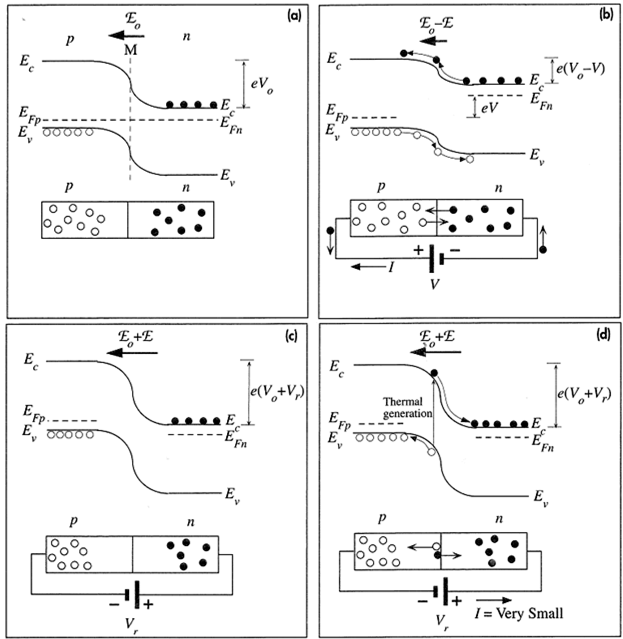
\includegraphics[width=0.6\linewidth]{images/pndiode.png}
    \caption{Energy band diagrams for a $pn$ junction (a) open circuit, (b) forward bias, (c) reverse bias, (d) thermal generation of electron-hole pairs.}
    \label{fig:pndiode}
\end{figure}

\paragraph{Forward bias}
The diode equation for forward bias is
\begin{equation}
    J = J_0 \left(e^{\frac{eV}{kT}} -1\right)
\end{equation}

\paragraph{Reverse bias}
Under reverse bias, the barrier is increased to $e (V_0 + V_r)$, which leads
to a separation of $e^-$ and $h^+$ and a very small reverse current.

\paragraph{Thermal generation of electron-hole pairs}
The thermal generation of electron-hole pairs leads to a small reverse current.

\subsection{Light emitting diodes (LED)}
A LED is a pn junction diode made from \emph{direct} bandgap semiconductors like GaAs.
The phenomenon of light emission from electron-hole-pair (EHP) recombination 
as a result of minority carrier injection is called \emph{injection electroluminescence}. 
To allow photons to escape, the p-layer must be thin enough.
The photons have an energy $h\nu \approx E_g$.

%TODO add relevant graphics

The LED efficiency is 
\begin{equation}
    \eta_{\mathrm{ext}} = \frac{P_{\mathrm{out} (\text{optical})}}{I V} \cdot \SI{100}{\percent}
\end{equation}

\paragraph{Heterojunction high-intensity LEDs}
A junction between two different bandgap semiconductors is called heterojunction.
A typical double heterostructure LED is shown in Fig.~\ref{fig:heterojunction_led}

\begin{figure}[ht!]
    %TODO: oh my god - draw this in TikZ!!!
    \centering
    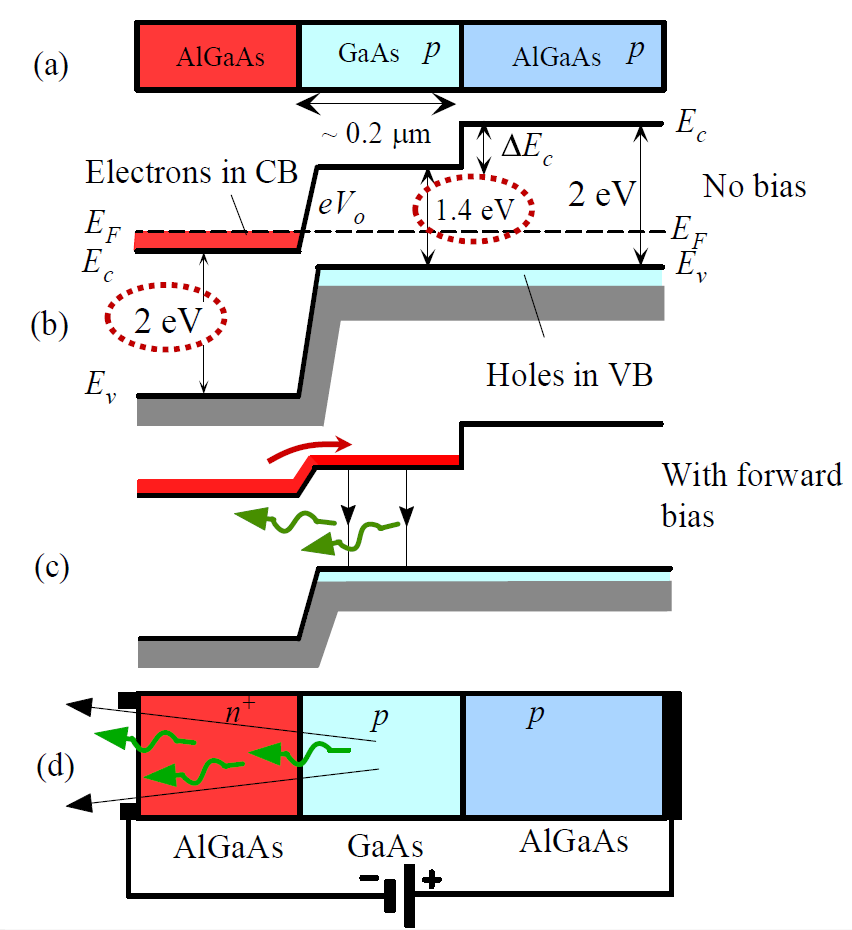
\includegraphics[width=0.4\linewidth]{images/heterojunction_led.png}
    \caption{(a) double heterostructure diode, (b) energy band diagram, (c) and (d) forward bias}
    \label{fig:heterojunction_led}
\end{figure}

The electrons are confined by the potential step between GaAs and AlGaAs to the right.
The photons escape reabsorption because the bandgap in AlGaAs is larger.

\subsection{Solar cells}
Solar cells have a very narrow and more heavily doped $n$-region.
The illumination is through the $n$-side.
Due to the asymmetry, the depletion region and the space charge layer (SCL)
extend primarily into the $p$-side. 

\begin{figure}[ht!]
    \centering
    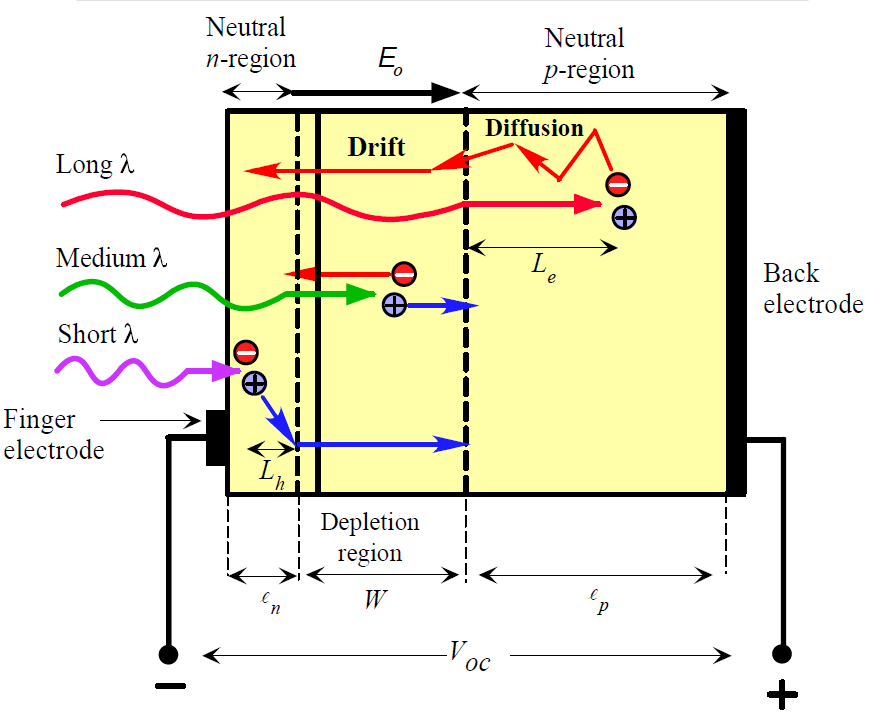
\includegraphics[width=0.5\linewidth]{images/solar_cell.png}
    \caption{Principle of operation of the solar cell}
\end{figure}

Photons form electron-hole-pairs, which are separated by the built-in field $E_0$.
This leads to an open circuit voltage with the $p$-side positive with respect to
the $n$-side.

Long-wavelength photons are absorbed in the neutral $p$-region where there is no
electric field. 
The mean diffusion length $L_e=\sqrt{2D_e\tau_e}$ where $\tau_e$ is the
recombination lifetime of the electron and $D_e$ is its diffusion coefficient.
This gives the active volume
\begin{equation}
    L_h + W + L_e
\end{equation}

Crystalline silicon has a bandgap of \SI{1.1}{\electronvolt} which corresponds
to a threshold wavelength of \SI{1.1}{\micro\meter}, i.e. wavelengths above this
are wasted, this is about \SI{25}{\percent}. 
Together with EHP recombination losses (about \SI{40}{\percent} near the surface)
this leads to the efficiency of about \SI{45}{\percent}.

When driving a load R, $I_d = I_0 \left( e^{\frac{eV}{\eta k T}}-1 \right)$.

The Fill factor $FF$ is a measure of closeness of the IV curve to rectangular shape.
\begin{equation}
    FF = \frac{I_m V_m}{I_{\text{short-circuit}} V_{\text{open-circuit}}} \approx 70 \ldots 85 \%
\end{equation}
